%! Author = paulsen
%! Date = 12.09.23

\begin{frame}{Installation}
    \section{Installation}\label{sec:installation}
\end{frame}

\begin{frame}{VirtualBox}
    \subsection{VirtualBox}\label{subsec:VirtualBox}
    Öffne Virtual Box und klicke auf "New".
    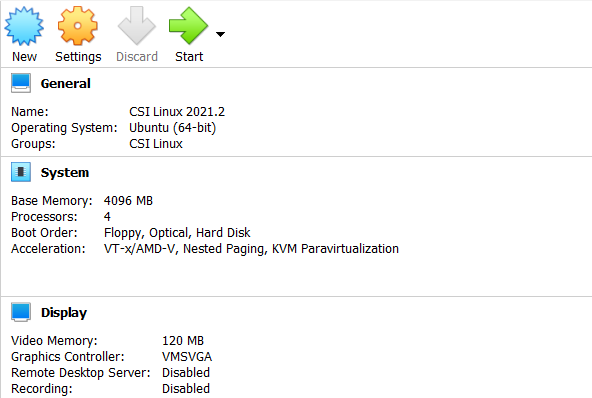
\includegraphics[width=10cm]{VirtualBox_1}
\end{frame}

\begin{frame}{VirtualBox}
    Gebe Namen und Installationsort ein.
    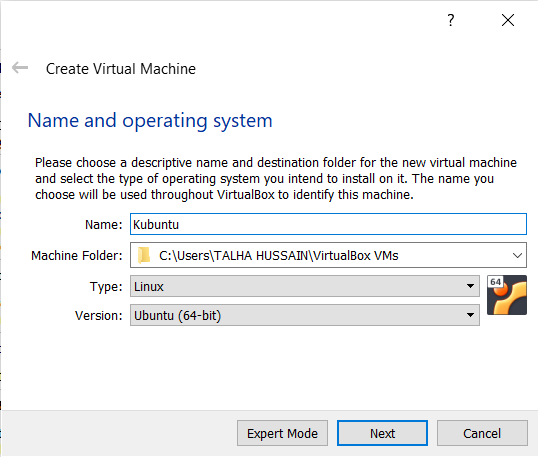
\includegraphics[width=10cm]{VirtualBox_2}
\end{frame}

\begin{frame}{VirtualBox}
    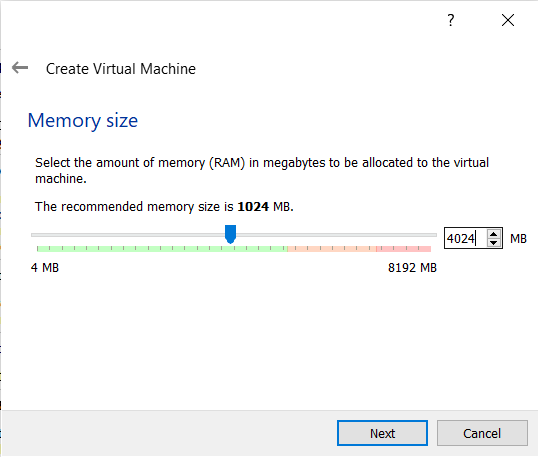
\includegraphics[width=10cm]{VirtualBox_3}
\end{frame}

\begin{frame}{VirtualBox}
    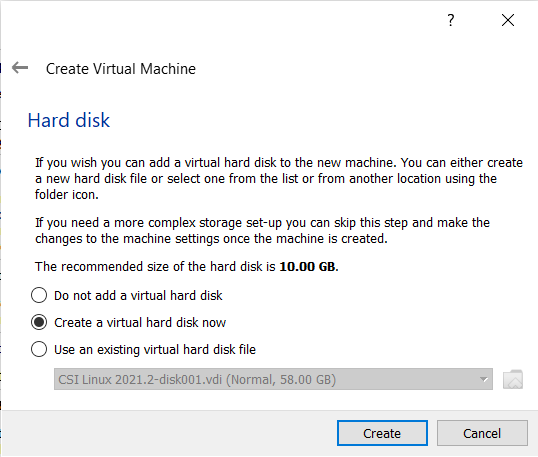
\includegraphics[width=10cm]{VirtualBox_4}
\end{frame}

\begin{frame}{VirtualBox}
    Wähle VDI aus
    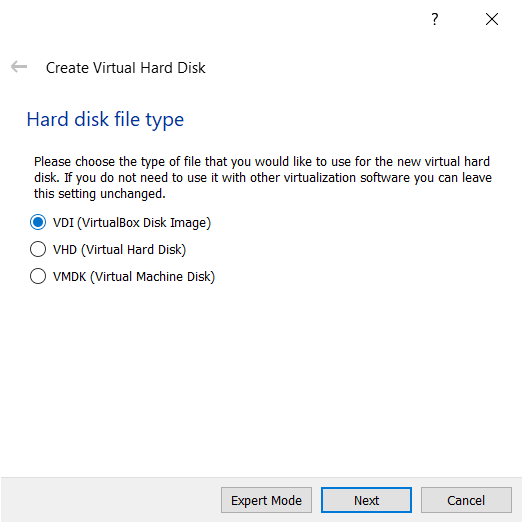
\includegraphics[width=10cm]{VirtualBox_5}
\end{frame}

\begin{frame}{VirtualBox}
    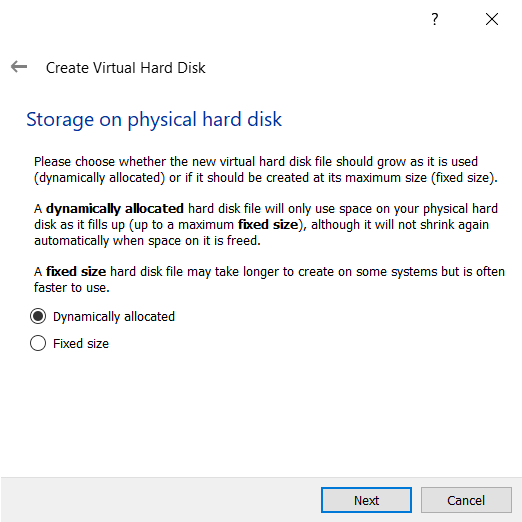
\includegraphics[width=10cm]{VirtualBox_6}
\end{frame}

\begin{frame}{VirtualBox}
    Füge eine Virtuelle Festplatte mit 10-20GB hinzu.
    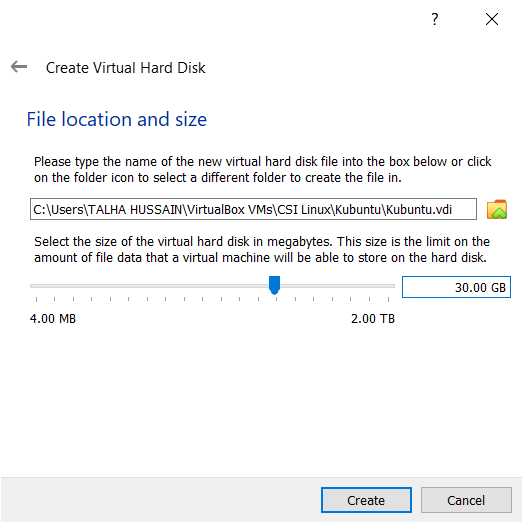
\includegraphics[width=10cm]{VirtualBox_7}
\end{frame}

\begin{frame}{VirtualBox}
    Gehe in den Einstellungen der VM auf "Storage" und wähle die ISO-Datei aus.
    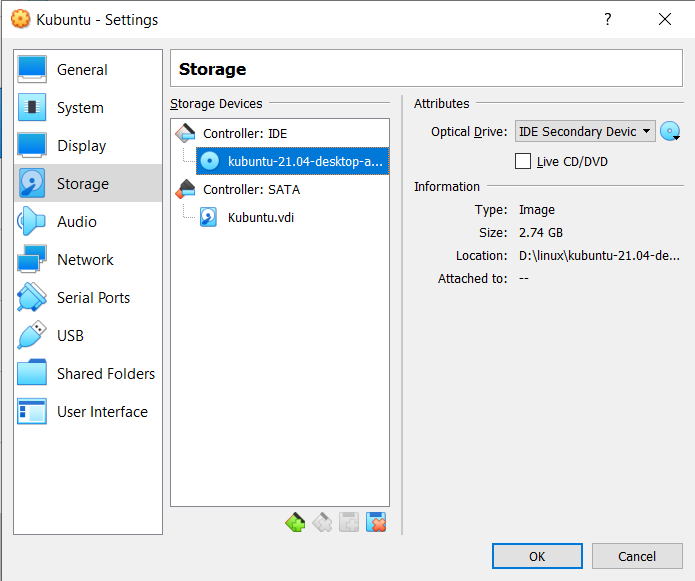
\includegraphics[width=8.5cm]{VirtualBox_8}
\end{frame}

\begin{frame}{Setup}
    \subsection{Setup}\label{subsec:setup}
    Beginne den Install-Prozess mit dem Starten der VM und wähle "Kubuntu" aus.
    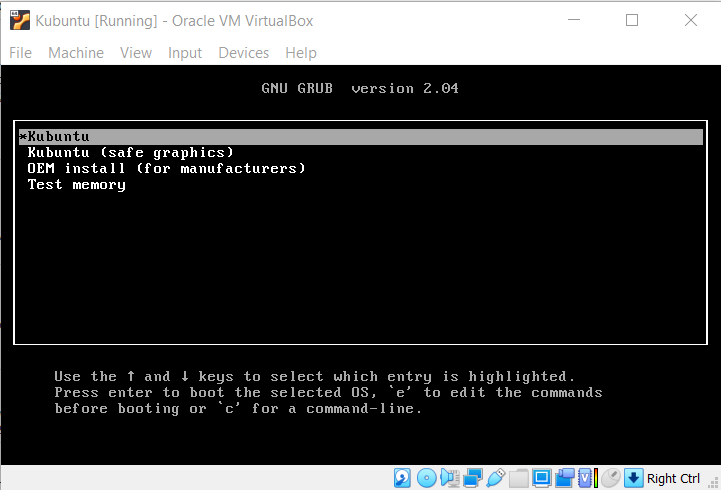
\includegraphics[width=9cm]{Install_1}
\end{frame}

\begin{frame}{Setup}
    Nach Starten des Live-Systems öffnen wir den grafischen Installer.
    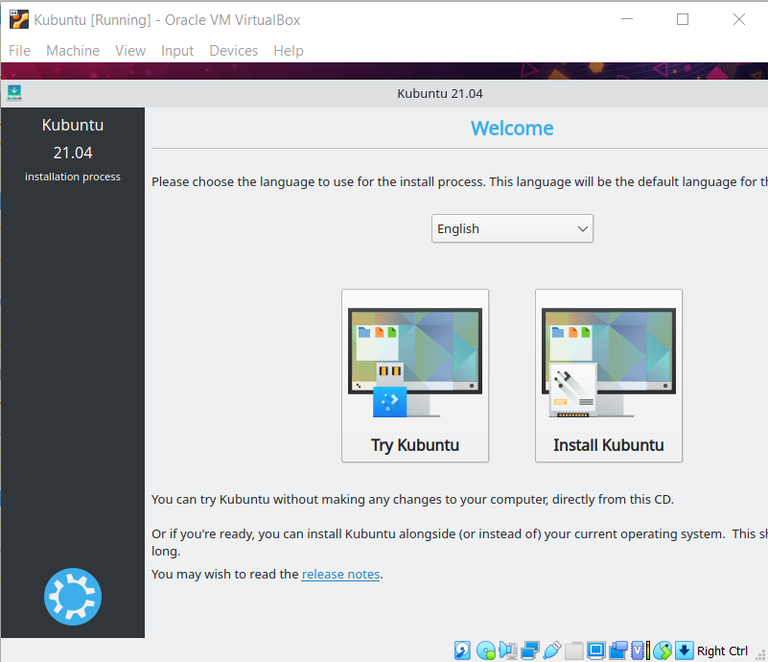
\includegraphics[width=9cm]{Install_2}
\end{frame}

\begin{frame}{Setup}
    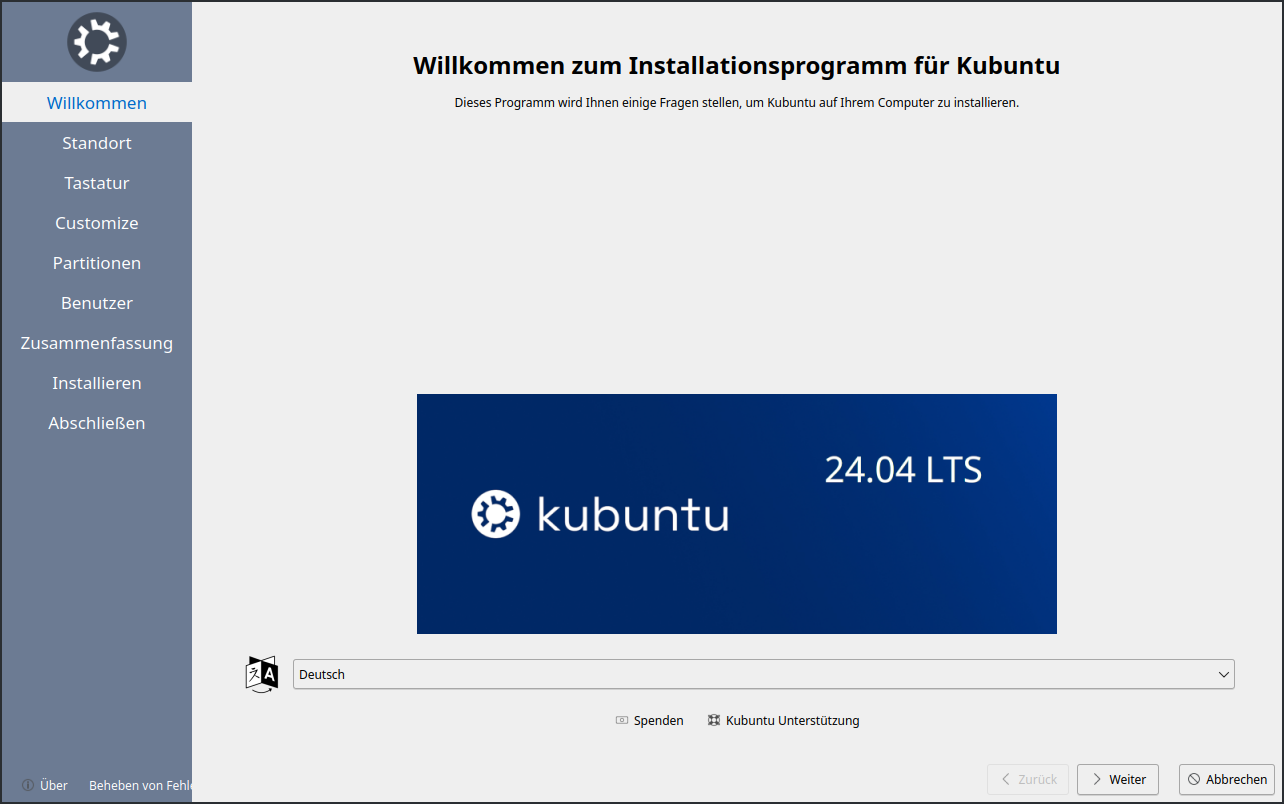
\includegraphics[width=10cm]{Install_3}
\end{frame}

\begin{frame}{Setup}
    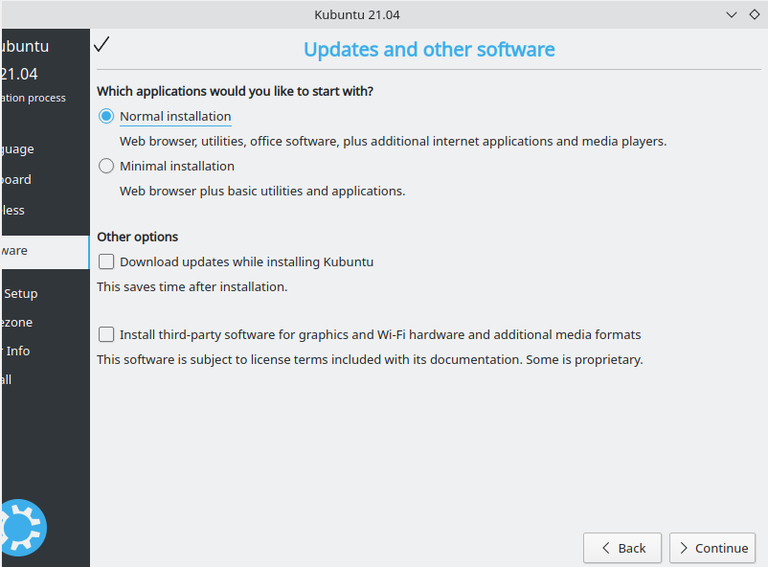
\includegraphics[width=10cm]{Install_4}
\end{frame}

\begin{frame}{Setup}
    Wähle die "Ganze Festplatte" als Option.
    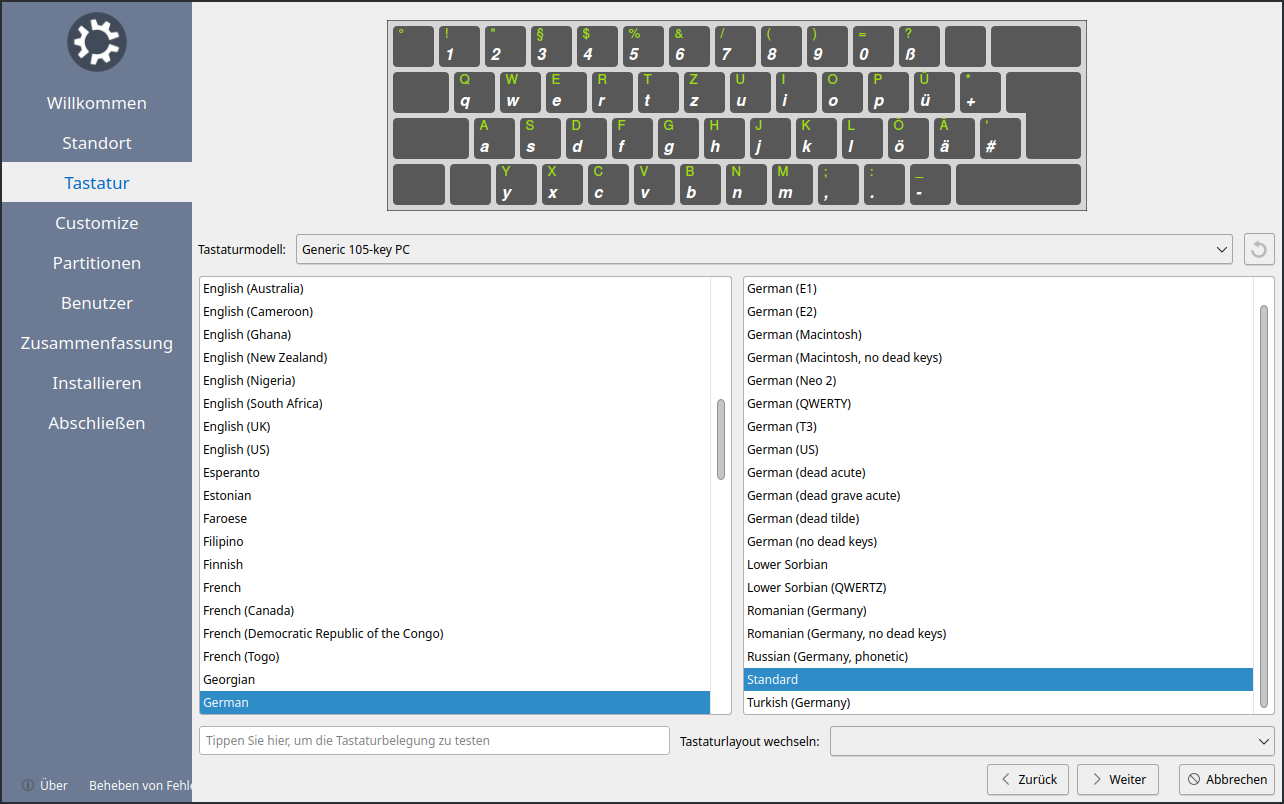
\includegraphics[width=9cm]{Install_5}
\end{frame}

\begin{frame}{Setup}
    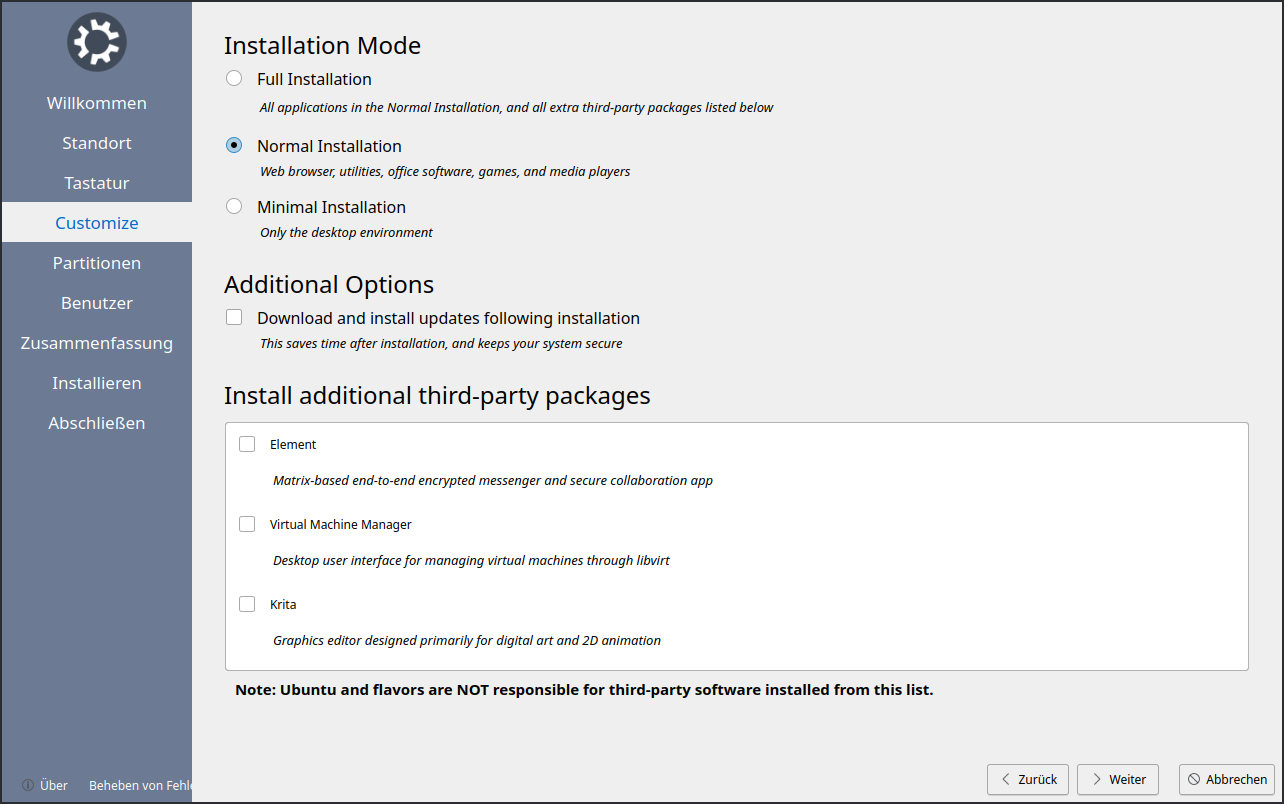
\includegraphics[width=10cm]{Install_6}
\end{frame}

\begin{frame}{Setup}
    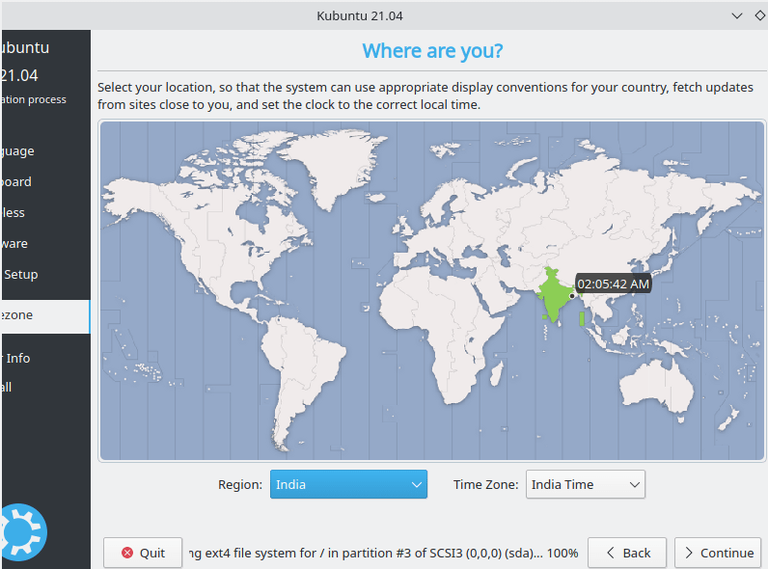
\includegraphics[width=10cm]{Install_7}
\end{frame}

\begin{frame}{Setup}
    Erstelle deinen Benutzer und wähle ein, für dich leicht zu merkendes, Passwort.
    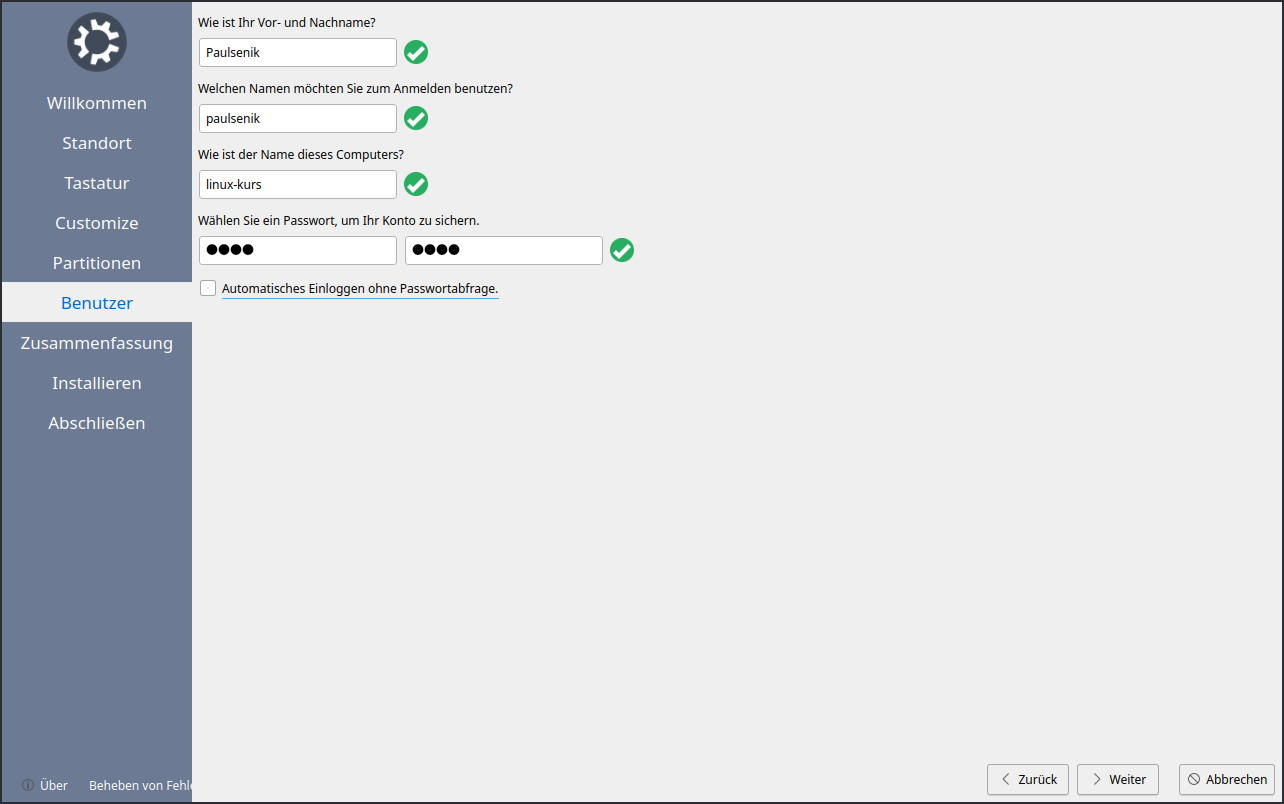
\includegraphics[width=9cm]{Install_8}
\end{frame}

\begin{frame}{Setup}
    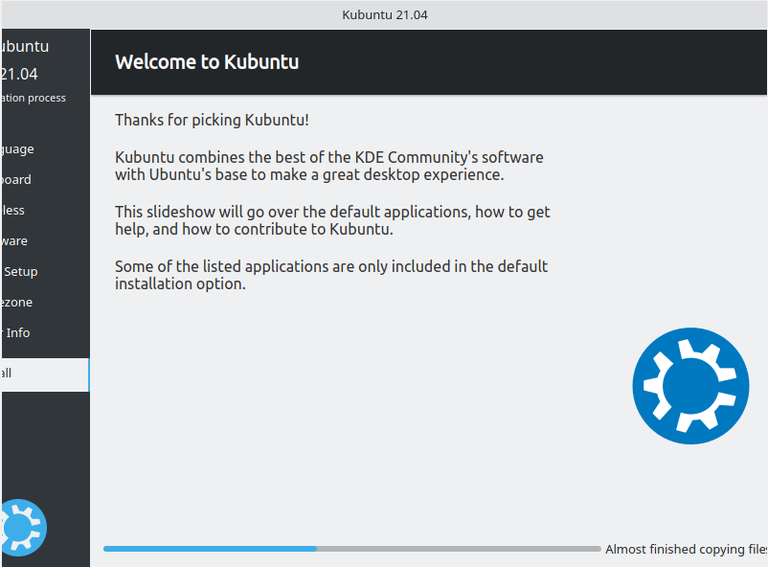
\includegraphics[width=9cm]{Install_9}
    \newline
    Starte die VM nach Fertigstellung neu.
\end{frame}